\subsubsection{Raman Spectroscopy of Graphene}

The Raman spectrum of graphene has three major peaks which are called for historical reasons $D$, $G$ and $2D$ as seen in figure~\ref{fig:dispersion}. While the $D$ peak is activated by defects in the graphene lattice the $G$ and $2D$ peaks are also present in pristine graphene~\cite{Ferrari2013}.

\begin{figure}[!h]
  \centering
  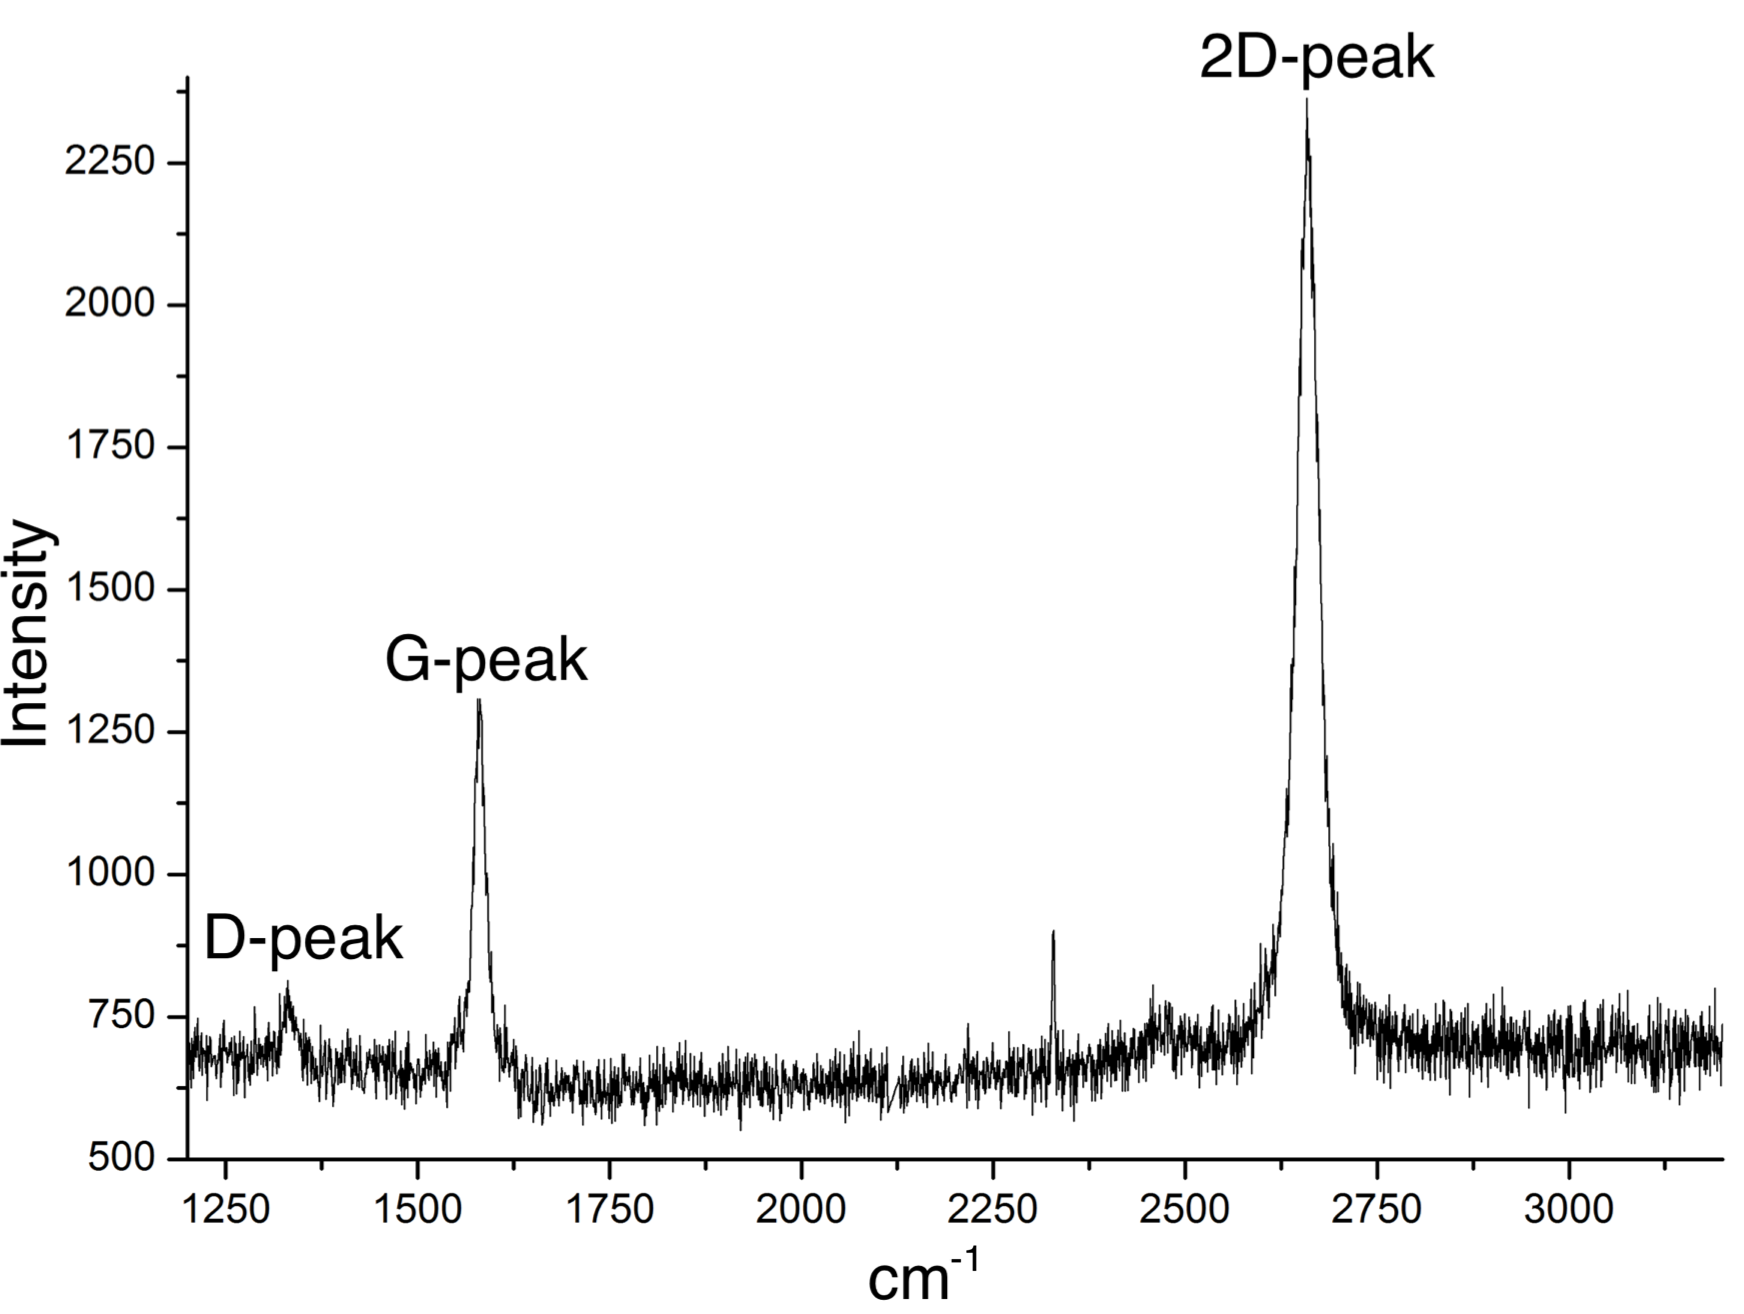
\includegraphics[width=0.5\textwidth]{./images/graphene-raman.png}
  \caption{The Raman spectrum of graphene showing the $D$, $G$ and $2D$ modes (adapted from \cite{Ferrari2013}).}
  \label{fig:dispersion}
\end{figure}

Similar to the electronic band structure of graphene it is also possible to define a phononic band structure as shown in figure~\ref{fig:phonons}. Due to its two-atom unit cell the phonon dispersion relation has three optical (O) and three acoustic branches (A). The phonon modes perpendicular to the plane are called out-of-plane (o) in contrast to in-plane modes (i). For further classification vibrations perpendicular and parallel to the axis of the two atoms in the unit cell are called transverse (T) and longitudinal (L).

\begin{figure}[!h]
  \centering
  \begin{subfigure}[t]{0.7\textwidth}
    \caption{}
    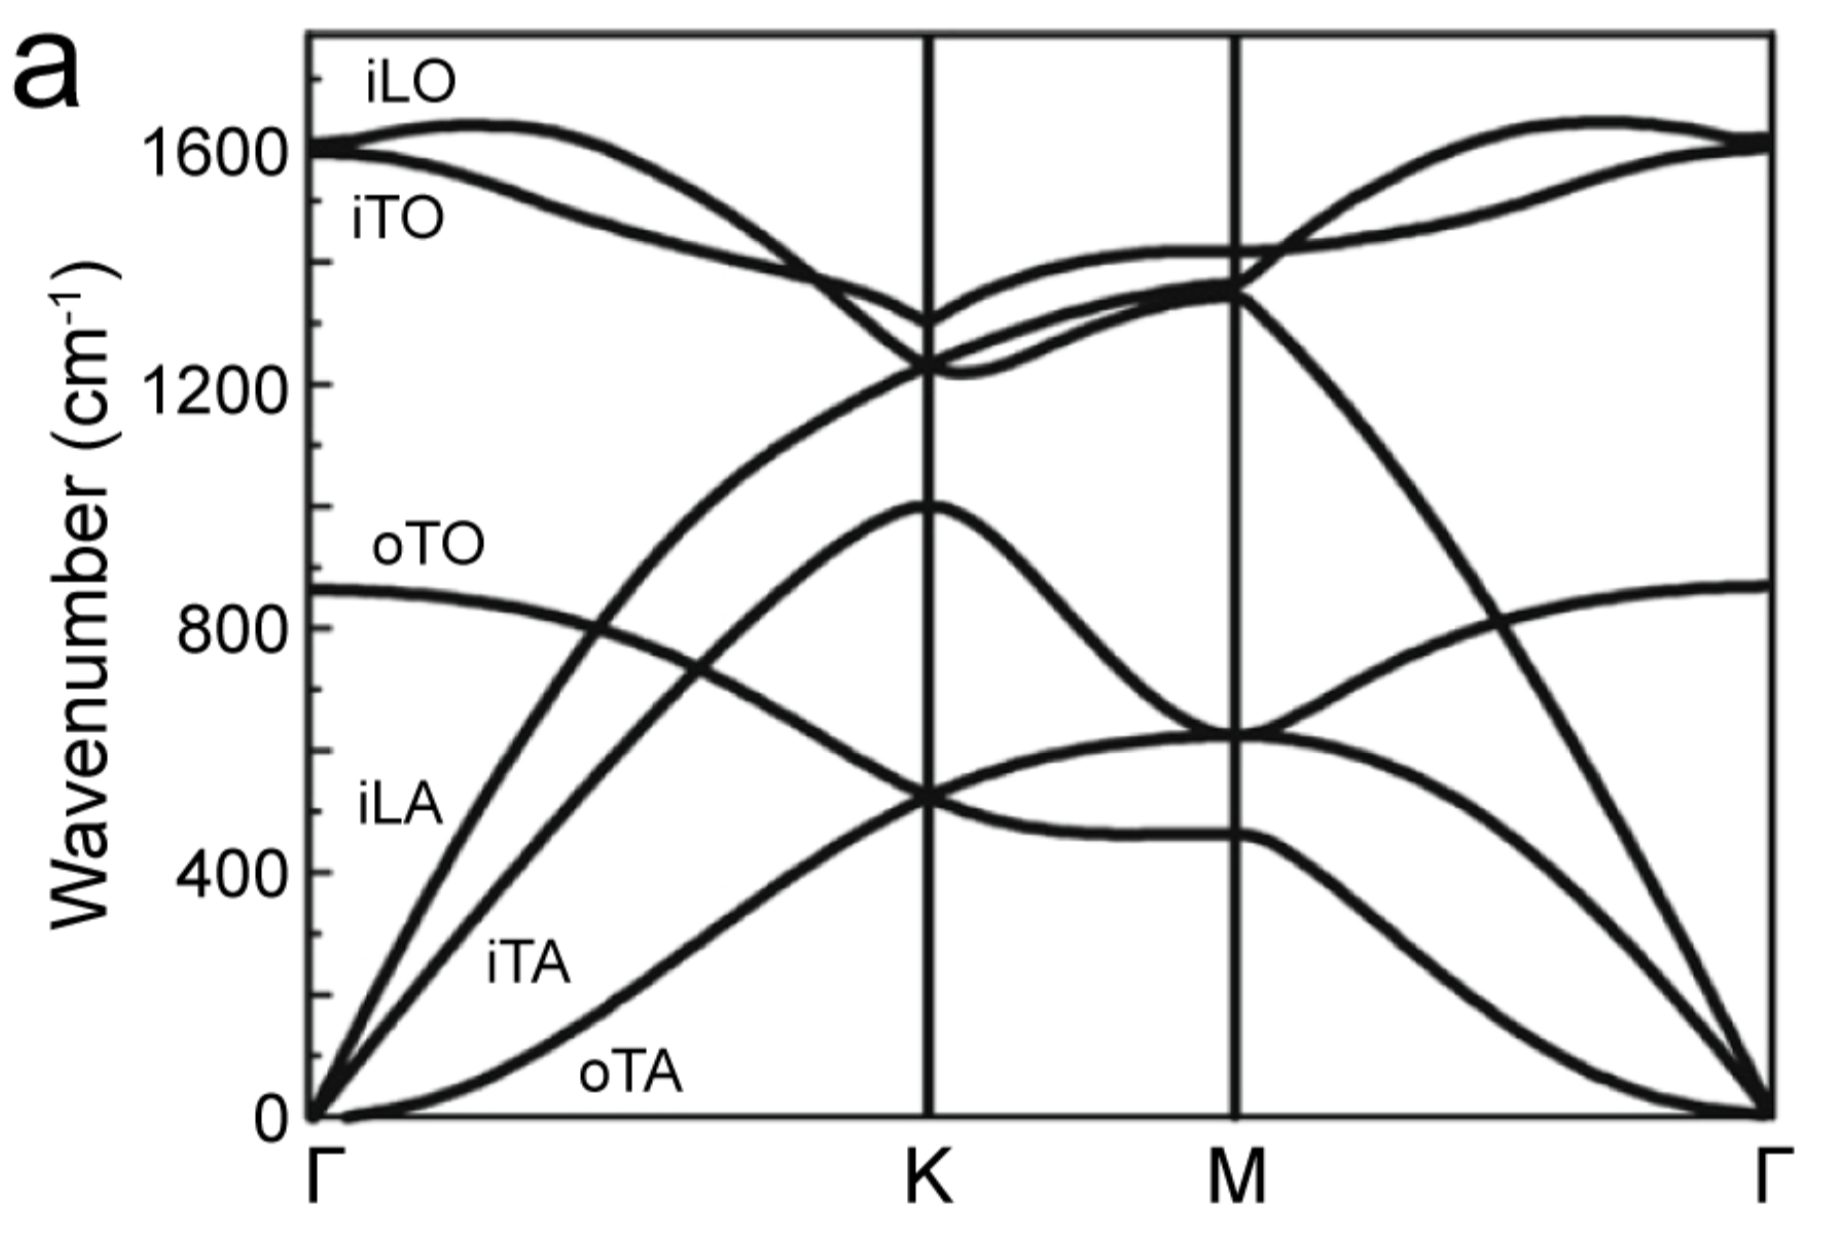
\includegraphics[width=\textwidth]{./images/phonon-modes.png}
  \end{subfigure}
  ~
  \begin{subfigure}[t]{0.25\textwidth}
    \begin{subfigure}[t]{\textwidth}
      \centering
      \caption{}
      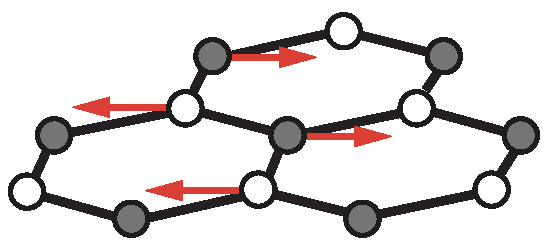
\includegraphics[width=\textwidth]{./images/g-mode-phonon.pdf}
      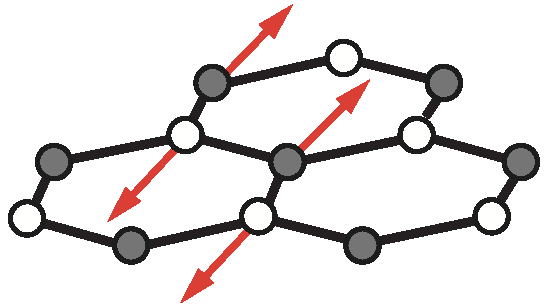
\includegraphics[width=\textwidth]{./images/g-mode-phonon-2.pdf}
    \end{subfigure}
    \begin{subfigure}[t]{\textwidth}
      \centering
      \caption{}
      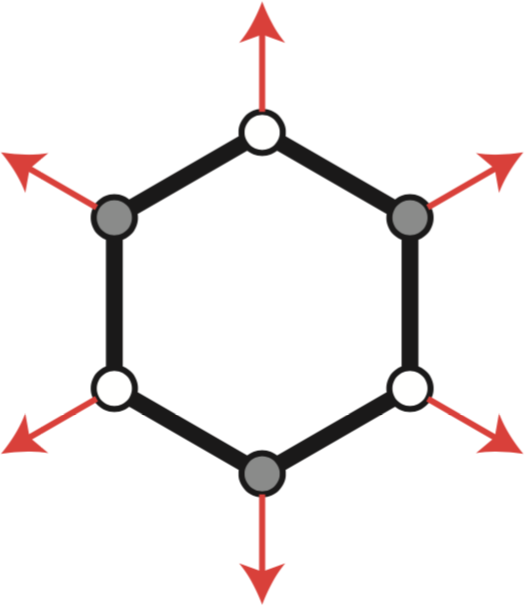
\includegraphics[width=0.7\textwidth]{./images/2d-mode-phonon.png}
    \end{subfigure}
  \end{subfigure}
  \caption{\textbf{(a)} Calculated phonon dispersion relation of graphene along the $\Gamma$-$K$-$M$-$\Gamma$-direction with six phonon branches (figure adapted from \cite{Malard2009}). \textbf{(b)} The two optical phonons (iLO and iTO) at the $\Gamma$-point causing the $G$ peak in graphene's Raman spectrum ($E_{2g}$ symmetry) (adapted from \cite{Ferrari2013}). \textbf{(c)} Phonon at $K$ causing the $2D$-peak in graphene's Raman spectrum ($A_1$ symmetry) (adapted from \cite{Ferrari2013}).}
  \label{fig:phonons}
\end{figure}

\newpage

\begin{figure}[!h]
  \centering
  \begin{subfigure}[t]{0.2\textwidth}
    \caption{}
    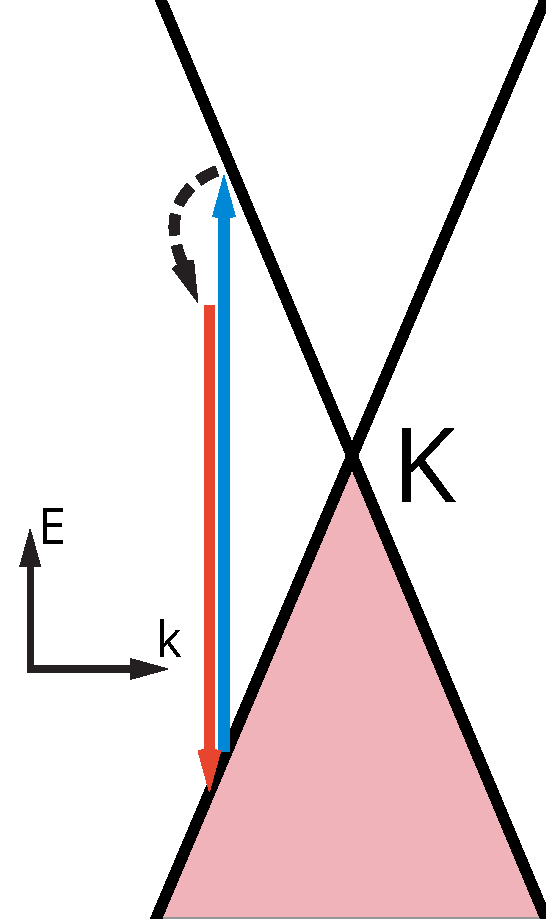
\includegraphics[width=\textwidth]{./images/g-mode.pdf}
  \end{subfigure}
  \qquad
  \begin{subfigure}[t]{0.45\textwidth}
    \caption{}
    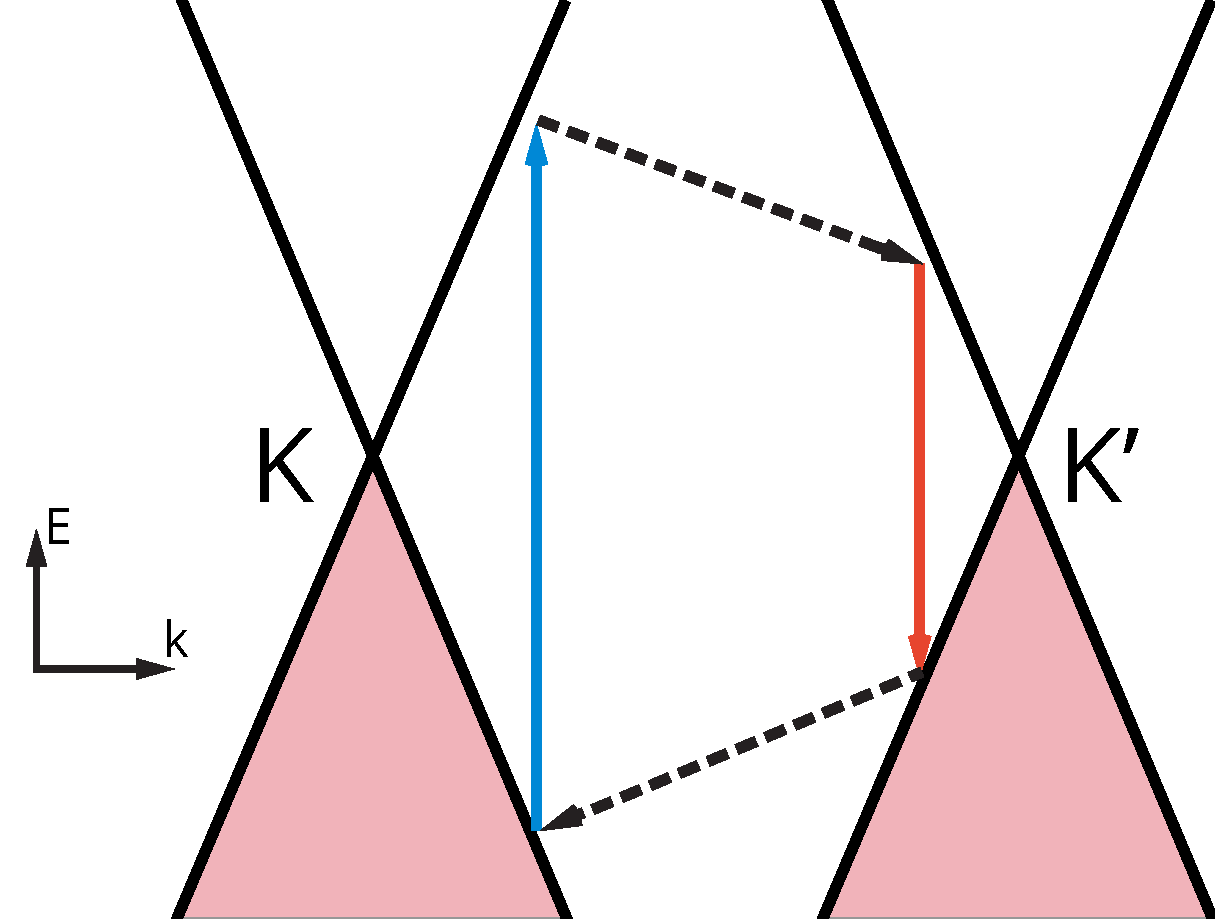
\includegraphics[width=\textwidth]{./images/2d-mode.pdf}
  \end{subfigure}
  \caption{Raman scattering processes for the $G$ and $2D$ peak of graphene. The band structure close to the K points is approximated as cones. \textbf{(a)} A photon is absorbed (blue arrow), scatters with a phonon (dashed arrow) and is then emitted with a lower frequency (red arrow), causing the $G$ peak in graphene's Raman spectrum (adapted from \cite{Ferrari2013}). \textbf{(b)} A photon is absorbed (blue arrow), then scatters with two phonons (dashed arrows) and is emitted at a lower frequency (red arrow), causing the $2D$ peak. This is the most prominent feature of graphene's Raman spectrum (adapted from \cite{Ferrari2013}).}
  \label{fig:raman-modes}
\end{figure}

The most prominent feature in the Raman spectrum of graphene is the $2D$ peak which is the $D$ peak overtone at $\sim$ \SI{2700}{cm^{-1}}. It is a second-order Raman mode that appears because of a double-resonance process\cite{double-resonance} (see figure~\ref{fig:raman-modes}). Two iTO phonons at the $K$ point with opposite wavevectors are involved in the scattering process to satisfy the momentum conservation as shown in figure~\ref{fig:raman-modes}. This mode does not require a defect for activation and is therefore always visible in graphene's Raman spectrum.

The G peak at \SI{1582}{cm^{-1}} is the only first-order Raman mode of graphene. It belongs to the iLO and iTO phonon branches at the $\Gamma$ point \cite{Ferrari2013}. This corresponds to vibrations of the two sublattices against each other. In group theory it belongs to the two-dimensional $E_{2g}$ representation~\cite{yucordona}.
